\documentclass[tikz,border=8pt]{standalone}
\usepackage{helvet}
\renewcommand{\familydefault}{\sfdefault}
\usetikzlibrary{arrows.meta,calc,decorations.pathmorphing,positioning}
\begin{document}
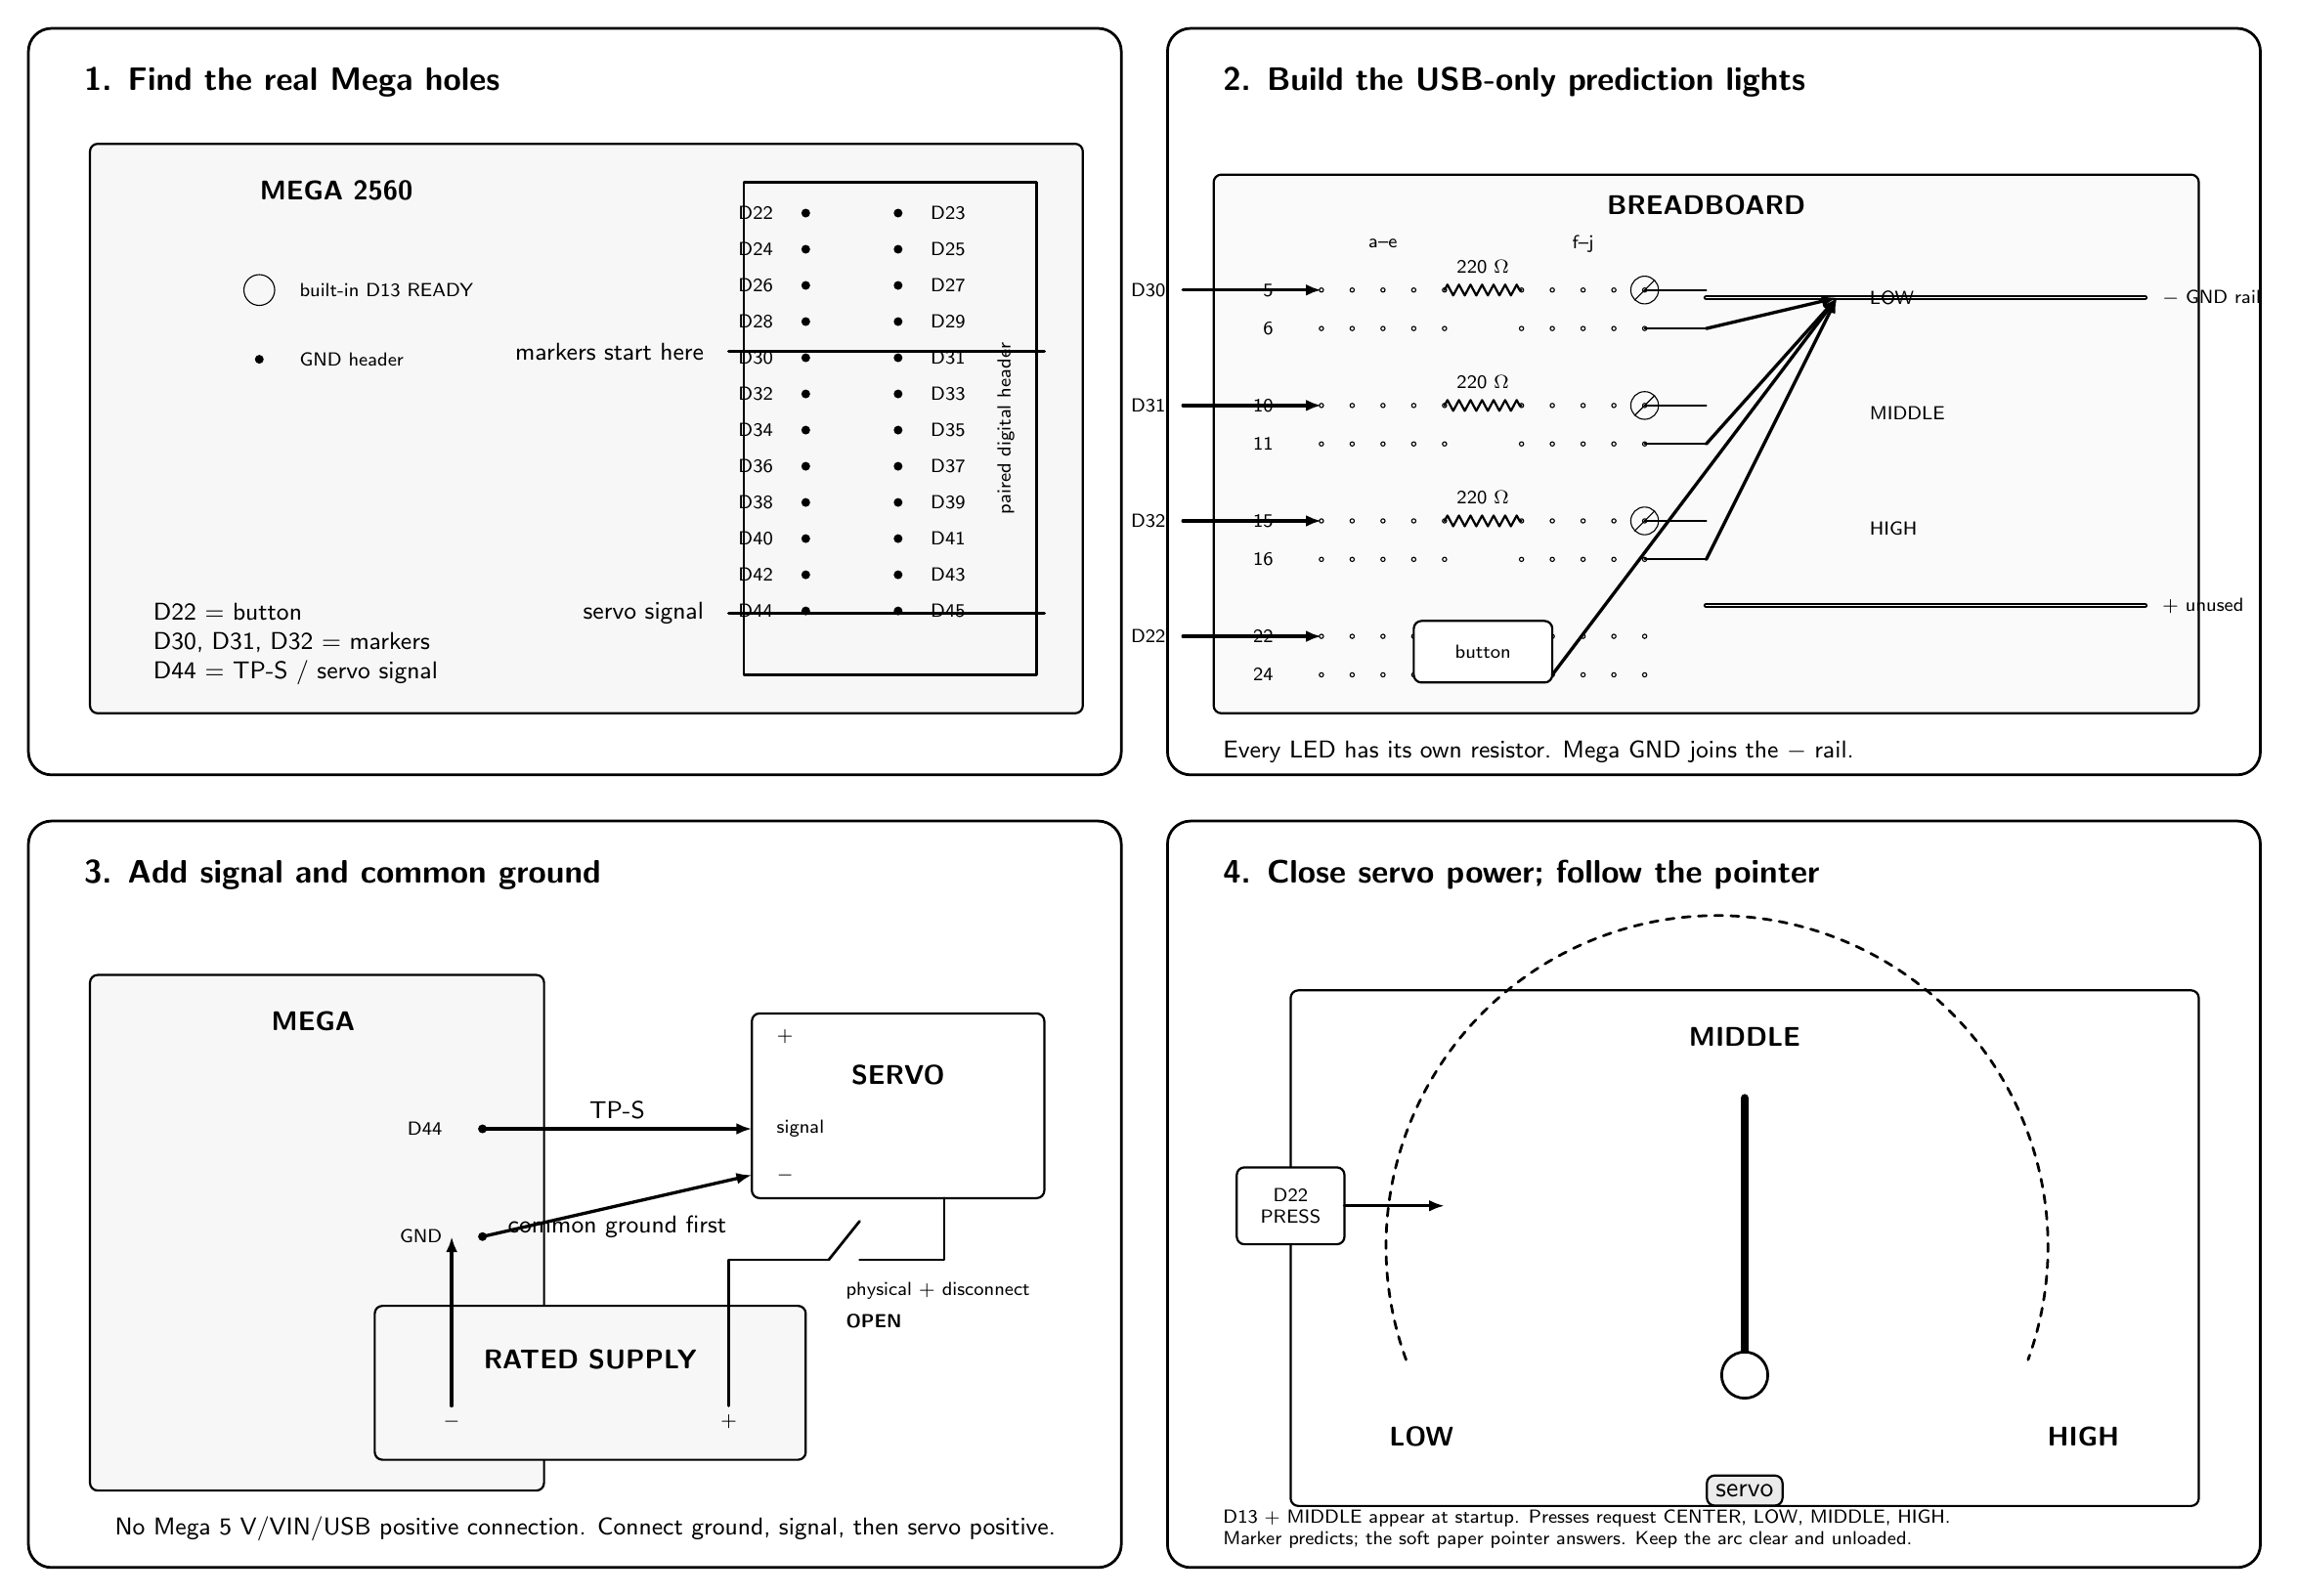
\begin{tikzpicture}[x=1mm,y=1mm,line cap=round,line join=round,
  wire/.style={line width=1.2pt,-{Latex[length=2mm]}},
  part/.style={draw,line width=.8pt,rounded corners=1mm,fill=white},
  hole/.style={circle,fill=black,inner sep=1.15pt},
  note/.style={font=\small},
  tinylabel/.style={font=\scriptsize}]

% Four sheet panels.
\foreach \x/\y in {0/103,148/103,0/0,148/0}
  \draw[line width=1pt,rounded corners=3mm] (\x,\y) rectangle ++(142,97);

\node[anchor=west,font=\bfseries\large] at (6,193) {1. Find the real Mega holes};
\node[anchor=west,font=\bfseries\large] at (154,193) {2. Build the USB-only prediction lights};
\node[anchor=west,font=\bfseries\large] at (6,90) {3. Add signal and common ground};
\node[anchor=west,font=\bfseries\large] at (154,90) {4. Close servo power; follow the pointer};

% Plate 1: credible Mega paired header locator.
\draw[part,fill=black!3] (8,111) rectangle (137,185);
\node[font=\bfseries] at (40,179) {MEGA 2560};
\draw (30,166) circle (2);
\node[tinylabel,anchor=west] at (34,166) {built-in D13 READY};
\node[hole] at (30,157) {};
\node[tinylabel,anchor=west] at (34,157) {GND header};
\draw[line width=.8pt] (93,116) rectangle (131,180);
\node[rotate=90,font=\scriptsize] at (127,148) {paired digital header};
\foreach \row/\leftpin/\rightpin in {
  0/22/23,1/24/25,2/26/27,3/28/29,4/30/31,5/32/33,
  6/34/35,7/36/37,8/38/39,9/40/41,10/42/43,11/44/45}
{
  \pgfmathsetmacro{\yy}{176-\row*4.7}
  \node[hole] at (101,\yy) {};
  \node[hole] at (113,\yy) {};
  \node[tinylabel,anchor=east] at (98,\yy) {D\leftpin};
  \node[tinylabel,anchor=west] at (116,\yy) {D\rightpin};
}
\draw[line width=1.2pt] (91,158) -- (132,158);
\node[note,anchor=east] at (89,158) {markers start here};
\draw[line width=1.2pt] (91,124) -- (132,124);
\node[note,anchor=east] at (89,124) {servo signal};
\node[note,align=left,anchor=west] at (15,120)
  {D22 = button\\D30, D31, D32 = markers\\D44 = TP-S / servo signal};

% Plate 2: breadboard with numbered rows and explicit component topology.
\draw[part,fill=black!2] (154,111) rectangle (282,181);
\node[font=\bfseries] at (218,177) {BREADBOARD};
\foreach \r/\yy in {5/166,6/161,10/151,11/146,15/136,16/131,22/121,24/116}
{
  \node[tinylabel,anchor=east] at (163,\yy) {\r};
  \foreach \xx in {168,172,176,180,184,194,198,202,206,210}
    \node[circle,draw,inner sep=.55pt] at (\xx,\yy) {};
}
\node[tinylabel] at (176,172) {a--e};
\node[tinylabel] at (202,172) {f--j};
\draw[double,line width=.7pt] (218,165) -- (275,165);
\draw[double,line width=.7pt] (218,125) -- (275,125);
\node[tinylabel,anchor=west] at (276,165) {$-$ GND rail};
\node[tinylabel,anchor=west] at (276,125) {$+$ unused};

% Three resistor/LED chains: D pin -> row n -> resistor across gutter -> LED to next row -> GND.
\foreach \pin/\yy/\nextyy/\name in {30/166/161/LOW,31/151/146/MIDDLE,32/136/131/HIGH}
{
  \draw[wire] (150,\yy) -- (168,\yy);
  \node[tinylabel,anchor=east] at (149,\yy) {D\pin};
  \draw[line width=.8pt,decorate,decoration={zigzag,segment length=1.5mm,amplitude=.7mm}]
    (184,\yy) -- (194,\yy);
  \node[tinylabel] at (189,\yy+3) {220 $\Omega$};
  \draw[line width=.8pt] (210,\yy) -- (218,\yy);
  \draw[line width=.8pt] (210,\nextyy) -- (218,\nextyy);
  \draw (210,\yy) circle (1.8);
  \draw (208.7,\yy-1.3) -- (211.3,\yy+1.3);
  \draw[wire] (218,\nextyy) -- (235,165);
  \node[tinylabel,anchor=west] at (238,\yy-1) {\name};
}
% Button on rows 22/24, D22 and ground.
\draw[wire] (150,121) -- (168,121);
\node[tinylabel,anchor=east] at (149,121) {D22};
\draw[part] (180,115) rectangle (198,123);
\node[tinylabel] at (189,119) {button};
\draw[wire] (198,116) -- (235,165);
\node[note,anchor=west] at (154,106) {Every LED has its own resistor. Mega GND joins the $-$ rail.};

% Plate 3: power and signal domains.
\draw[part,fill=black!3] (8,10) rectangle (67,77);
\node[font=\bfseries] at (37,71) {MEGA};
\node[hole] at (59,57) {};\node[tinylabel,anchor=east] at (55,57) {D44};
\node[hole] at (59,43) {};\node[tinylabel,anchor=east] at (55,43) {GND};
\draw[part] (94,48) rectangle (132,72);
\node[font=\bfseries] at (113,64) {SERVO};
\node[tinylabel,anchor=west] at (96,57) {signal};
\node[tinylabel,anchor=west] at (96,51) {$-$};
\node[tinylabel,anchor=west] at (96,69) {$+$};
\draw[wire] (59,57) -- node[above,note]{TP-S} (94,57);
\draw[wire] (59,43) -- node[below,note]{common ground first} (94,51);
\draw[part,fill=black!3] (45,14) rectangle (101,34);
\node[font=\bfseries] at (73,27) {RATED SUPPLY};
\node[tinylabel] at (55,19) {$-$};
\node[tinylabel] at (91,19) {$+$};
\draw[wire] (55,21) -- (55,43);
\draw[line width=1pt] (91,21) -- (91,40) -- (104,40);
\draw[line width=1pt] (108,40) -- (119,40) -- (119,48);
\draw[line width=1pt] (104,40) -- (108,45);
\node[tinylabel,anchor=west] at (105,36) {physical $+$ disconnect};
\node[tinylabel,anchor=west,font=\scriptsize\bfseries] at (105,32) {OPEN};
\node[note,align=left,anchor=west] at (10,5)
  {No Mega 5 V/VIN/USB positive connection. Connect ground, signal, then servo positive.};

% Plate 4: pointer card and expected states.
\draw[part] (164,8) rectangle (282,75);
\draw[dashed,line width=1pt] (179,27) arc[start angle=200,end angle=-20,radius=43];
\draw[line width=3pt] (223,25) -- (223,61);
\draw[fill=white,line width=1pt] (223,25) circle (3);
\node[font=\bfseries] at (181,17) {LOW};
\node[font=\bfseries] at (223,69) {MIDDLE};
\node[font=\bfseries] at (267,17) {HIGH};
\node[part,fill=black!8] at (223,10) {servo};
\draw[part] (157,42) rectangle (171,52);
\node[tinylabel,align=center] at (164,47) {D22\\PRESS};
\draw[wire] (171,47) -- (184,47);
\node[tinylabel,align=left,anchor=west] at (154,5)
  {D13 + MIDDLE appear at startup. Presses request CENTER, LOW, MIDDLE, HIGH.\\
   Marker predicts; the soft paper pointer answers. Keep the arc clear and unloaded.};

\end{tikzpicture}
\end{document}
